\documentclass[12pt, a4paper]{article}
\usepackage[utf8]{inputenc}
\usepackage{polski}
\usepackage{hyperref}
\usepackage{algorithm}% http://ctan.org/pkg/algorithms
\usepackage{algpseudocode}% http://ctan.org/pkg/algorithmicx
\usepackage[titletoc]{appendix}
\usepackage{graphicx}  
\usepackage{float}
\usepackage{placeins}
\usepackage{geometry}
\title{\textbf{Poszukiwanie największej kliki w~grafie}}
\author{Anna Stępień \\ Adam Stelmaszczyk}
\date{}
\setlength{\parindent}{0in}
\renewcommand\refname{Referencje}
\makeatletter\renewcommand{\ALG@name}{}

\newgeometry{tmargin=2.5cm, bmargin=2.5cm, lmargin=3cm, rmargin=3cm}

\begin{document}
\maketitle
\tableofcontents

\newpage
\section{Zadanie}

Kliką grafu nazywamy podgraf, w którym każde dwa wierzchołki są ze sobą połączone.
Maksymalną kliką nazywamy klikę, do której nie można dodać ani jednego wierzchołka więcej, tak aby razem z nią nadal tworzył klikę.
Największą kliką nazywamy klikę o~największej liczbie wierzchołków.
Celem zadania jest implementacja wybranego algorytmu znajdującego największa klikę w~grafie oraz analiza otrzymanych wyników.

\section{Założenia}
Realizowana aplikacja będzie pracowała w~trybie konsolowym i będzie przyjmowała pliki z danymi przekazane na strumień wejściowy.

W~projekcie zostanie wykorzystany zmodyfikowany algorytm Brona--Kerboscha \cite{bk}, dokładniej opisany w sekcji \ref{bron_kerbosch}.
Do implementacji zadania wykorzystany zostanie język Java.

\subsection{Dane wejściowe}
Wejściem dla algorytmu jest graf nieskierowany dany macierzą o~$n$~wierszach i~$n$~kolumnach:

\bigskip
$ 
\begin{array}{cccc}
q_{0,0} & q_{1,0} & \ldots & q_{n-1,0} \\
q_{0,1} & q_{1,1} & \ldots & q_{n-1,1} \\
\vdots  & \vdots  & \ddots & \vdots  \\
q_{0,n-1} & q_{1,n-1} & \ldots & q_{n-1,n-1} 
\end{array}
, q_{i,j} \in \{0,1\}, 0 \leq i,j < n
$
\bigskip

$q_{i,j}$ równe 0 oznacza, że wierzchołki i oraz j nie są połączone krawędzią. W~przeciwnym razie, wierzchołki są połączone.
\par\vspace{\baselineskip}
Macierz jest dana w pliku tekstowym, w którym kolejne $q_{i,j}$ w wierszu $j$ są
oddzielone co najmniej jednym znakiem białym. Przez znak biały rozumiemy
spację lub tabulator. $q_{i,j}$ różne od 0 będą traktowane jak 1.

Poniżej przedstawiono przykładowy, poprawny plik wejściowy.

\bigskip

$ 
\begin{array}{cccc}
0 & 1 & 0 & 0 \\
1 & 0 & 1 & 1 \\
0 & 1 & 0 & 1 \\
0 & 1 & 1 & 0
\end{array}
$
\bigskip

Kolejne $q_{i,j}$ w wierszu $j$ są oddzielone co najmniej jednym znakiem białym. 
Przez znak biały rozumiemy spację lub tabulator. $q_{i,j}$ różne od 0 będą traktowane jak 1.
\subsection{Dane wyjściowe}
Wyjściem jest niepusty zbiór numerów wierzchołków, które tworzą największą klikę w~podanym grafie. 
Wierzchołki numerujemy od 0 do $n-1$. W~grafie może istnieć więcej niż jedna największa klika.
W~takim przypadku algorytm zwróci pierwszą ze znalezionych klik.
\subsection{Sytuacje wyjątkowe}
Problemami, które mogą wystąpić podczas działania aplikacji są:
\begin{itemize}
	\item błędny format danych wejściowych,
	\item przepełnienie stosu spowodowane zbyt głębokim poziomem rekurencji.

\bigskip
W przypadku, gdy algorytm otrzyma na wejściu błędne dane np. liczba wierszy macierzy będzie niezgodna z zadeklarowaną na początku pliku z danymi, użytkownik zostanie poinformowany o zaistniałej sytuacji a dalsze działanie programu zostanie przerwane.

\bigskip
Ze względu na rekurencyjny charakter algorytmu Brona--Kerboscha może się zdarzyć, iż dla pewnych danych wejściowych algorytm nie będzie w stanie zwrócić wyniku ze względu na ograniczoną pojemność stosu.
Próbą rozwiązania tego problemu mogłaby być iteracyjna implementacja algorytmu.

\end{itemize}
\section{Algorytm}
\label{bron_kerbosch}
Algorytm Brona--Kerboscha jest rekurencyjnym algorytmem z nawrotami, który umożliwia poszukiwanie maksymalnych klik w zadanym grafie niezorientowanym.

Domyślnie algorytm zwraca wszystkie maksymalne kliki. W algorytmie wprowadzona zostanie zmiana, dzięki której zwracana będzie największa ze znalezionych maksymalnych klik, charakteryzująca się największą liczbą wierzchołków.

\subsection{Pseudokod}
Na poniższym listingu przedstawiona została podstawowa wersja algorytmu Brona--Kerboscha. 
\begin{algorithm}[!htb]
\caption{Algorytm Brona--Kerboscha (wersja podstawowa)}\label{bron1}
\begin{algorithmic}[1]
\State $compsub \gets \emptyset$
\State $candidates \gets V(G)$
\State $not \gets \emptyset$
\State $cliques \gets \emptyset$
\Function{bron\_kerbosch}{$compsub,candidates,not$}
	\If{$candidates = \emptyset$ \textbf{and} $not = \emptyset$}
		 \State $cliques \gets cliques \cup \{compsub\}$\Comment Maksymalna klika
	\Else
	\For{\textbf{each} $v$ in $candidates$}
		\State $candidates \gets candidates \setminus \{v\}$
		\State $new\_compsub \gets compsub \cup \{v\}$
		\State $new\_candidates \gets candidates \cap neighbors(v)$
		\State $new\_not \gets not \cap neighbors(v)$
		\State\Call{bron\_kerbosch}{$new\_compsub, new\_candidates, new\_not$}
		\State $compsub \gets compsub \cup \{v\}$
	\EndFor
	\EndIf
\EndFunction
\end{algorithmic}
\end{algorithm}

Poniżej przedstawiona została zmodyfikowana wersja algorytmu, która zostanie wykorzystana do realizacji zadania.
\begin{algorithm}[!htb]
\caption{Algorytm Brona--Kerboscha (wersja rozszerzona)}\label{bron2}
\begin{algorithmic}[1]
\State $compsub \gets \emptyset$
\State $candidates \gets V(G)$
\State $not \gets \emptyset$
\State $biggest\_clique \gets \emptyset$
\Function{bron\_kerbosch}{$candidates,not$}
	\If{$candidates = \emptyset$ \textbf{and} $not = \emptyset$}
		\If{$size(biggest\_clique) < size(compsub)$}
		 	\State $biggest\_clique \gets compsub$\Comment Największa klika
		 \EndIf
	\Else
	\State $pivot \gets vertex\_with\_maxdeg(candidates \cup not)$
	\State $candidates\_to\_check \gets candidates \setminus neighbors(pivot)$
	\For{\textbf{each} $v$ in $candidates\_to\_check$}
		\State $compsub \gets compsub \cup \{v\}$
		\State $candidates \gets candidates \setminus \{v\}$
		\State $new\_candidates \gets candidates \cap neighbors(v)$
		\State $new\_not \gets not \cap neighbors(v)$
		\State\Call{bron\_kerbosch}{$new\_candidates, new\_not$}
		\State $compsub \gets compsub \setminus \{v\}$
		\State $not \gets not \cup \{v\}$
	\EndFor
	\EndIf
\EndFunction
\end{algorithmic}
\end{algorithm}

\newpage
\subsection{Opis działania}
Istotą działania przedstawionego algorytmu jest utrzymywanie trzech rozłącznych zbiorów: $compsub$, $candidates$ oraz $not$.

Algorytm Brona--Kerboscha znajduje maksymalne kliki składające się ze wszystkich wierzchołków należących do zbioru $compsub$, niektórych należących do zbioru $candidates$, i z żadnego, który należy do zbioru $not$.

Poniżej przedstawiona została charakterystyka każdego ze zbiorów wykorzystywanych przez algorytm:
\begin{itemize}
	\item $compsub$ 
	
	do zbioru należą wszystkie wierzchołki grafu, które tworzą powstającą klikę.
	\item $candidates$
	
	do zbioru należą wierzchołki grafu, które mogą posłużyć do rozszerzenia zbioru $compsub$.
	\item $not$ 
	
	do zbioru należą te wierzchołki, które były już wcześniej wykorzystane do rozszerzenia zbioru $compsub$.
\end{itemize}

Należy zauważyć, iż wszystkie wierzchołki, które są połączone z każdym wierzchołkiem należącym do zbioru $compsub$ znajdują się albo w zbiorze $candidates$ albo $not$.

\bigskip
Zmodyfikowana wersja algorytmu Brona--Kerboscha wprowadza pojęcie wierzchołka zwrotnego (dalej oznaczanego $pivot$), który wybierany jest ze zbioru $candidates \cup not$ jako wierzchołek o największym stopniu.

\bigskip
W każdym rekurencyjnym wywołaniu algorytmu rozważane są wierzchołki należące do zbioru $candidates$. Jeśli zbiory $candidates$ i $not$ są puste, sprawdzane jest czy znaleziona maksymalna klika (oparta na wierzchołkach ze zbioru $compsub$) jest większa od największej dotychczas znalezionej kliki. Jeśli tak, to znaleziona klika staje się największą, w przeciwnym wypadku największa klika pozostawiana jest bez zmian.

W przypadku, gdy zbiory $candidates$ i $not$ nie są puste, dla każdego wierzchołka ze zbioru $candidates \setminus neighbors(pivot)$ następuje rekurencyjne wywołanie algorytmu, w którym bieżący wierzchołek $v$ dodawany jest do zbioru $compsub$ i usuwany ze zbioru $candidates$, a w zbiorach $candidates$ i $not$ pozostawiane są tylko te wierzchołki grafu, które są sąsiadami wierzchołka $v$. Następnie, wierzchołek $v$ jest dodawany do zbioru $not$ jako już wykorzystany do rozszerzenia kliki oraz usuwany ze zbioru $compsub$.

Wynikiem działania algorytmu jest zbiór $biggest\_clique$, który początkowo inicjowany jest jako zbiór pusty. W przypadku, gdy znaleziona zostanie największa klika, zbiór ten zawiera wierzchołki ją tworzące.

\subsection{Złożoność}
Pesymistyczna złożoność przedstawionego algorytmu wynosi $O(3^{n/3})$ i wynika z górnego ograniczenia na liczbę maksymalnych klik w grafie o n wierzchołkach.

\section{Struktury danych}
\paragraph{Graf}
Do reprezentacji grafu zostanie wykorzystana macierz sąsiedztwa, zaimplementowana jako dwuwymiarowa tablica wartości boolowskich.

\paragraph{Zbiory wierzchołków ($compsub$, $candidates$, $not$, $biggest\_clique$)}
Zbiory przechowujące wierzchołki zostaną zaimplementowane jako klasa $Vertices$ dziedzicząca po klasie $TreeSet$ języka Java.

\section{Testy}
Istotną częścią realizowanego zadania jest przeprowadzenie testów związanych zarówno z poprawnością zwracanych wyników jak również wpływem danych wejściowych na czas wykonania algorytmu.

\subsection{Badanie poprawności zwracanych wyników}
\label{igraph-testy}
Do weryfikacji poprawności zwracanych przez algorytm wyników zostanie wykorzystana biblioteka igraph\footnote{\url{http://igraph.sourceforge.net/}}, która udostępnia m.in funkcję wyznaczającą maksymalne kliki w zadanym grafie. Podczas testowania planujemy wykorzystać dane zwrócone przez bibliotekę igraph jako rozwiązania referencyjne, które następnie posłużą do porównania z wynikami otrzymanymi przez zaimplementowany algorytm. Rozwiązanie, a więc największa klika zwrócona przez algorytm jest poprawna wtedy, gdy znajduje się na liście rozwiązań referencyjnych.

Proces generowania rozwiązań referencyjnych oraz porównywania wyników zostanie zautomatyzowany.
\subsection{Badanie czasu wykonania dla różnych typów grafów}
Z punktu widzenia analizy zaimplementowanego algorytmu istotne jest zbadanie jego zachowania dla różnych typów grafów. W szczególności przeprowadzone zostaną eksperymenty na zestawach grafów o zróżnicowanej gęstości.

\section{Analiza zaimplementowanego algorytmu}
W ramach części badawczej projektu zrealizowane zostały dwa rodzaje testów: testy wykazujące poprawność implementacji algorytmu oraz testy badające jego zachowanie dla różnych typów grafów.

W obu eksperymentach wykorzystano następujące zestawy grafów:
\begin{itemize}
	\item zestaw grafów losowych o gęstości 0,1
	\item zestaw grafów losowych o gęstości 0,2
	\item zestaw grafów losowych o gęstości 0,3
    \item zestaw grafów losowych o gęstości 0,4
	\item zestaw grafów losowych o gęstości 0,5
	\item zestaw grafów losowych o gęstości 0,6
	\item zestaw grafów losowych o gęstości 0,7
	\item zestaw grafów losowych o gęstości 0,8
	\item zestaw grafów losowych o gęstości 0,9
	\item zestaw grafów pełnych
\end{itemize}
W każdym zestawie znalazły się grafy o liczbie wierzchołków: 10, 20, 30, 40, 50, 60, 70, 80, 90, 100.

Podczas analizy zbadane zostały dwa przypadki:
\begin{itemize}
	\item wpływ liczby wierzchołków dla grafów o ustalonej gęstości,
	\item wpływ gęstości dla grafów o ustalonej liczbie wierzchołków.
\end{itemize}

\subsection{Analiza poprawności działania algorytmu}
Przed przystąpieniem do właściwej analizy działania algorytmu została zweryfikowana poprawność jego implementacji. Do testowania poprawności działania programu wykorzystana została biblioteka igraph. Szczegółowy schemat testowania został przedstawiony w rozdziale \ref{igraph-testy}.
Testy zostały przeprowadzone na zestawie grafów opisanych na początku niniejszego rozdziału i nie wykazały błędów ani problemów z działaniem algorytmu.

\subsection{Analiza czasów wykonania algorytmu}
\label{testy}
Dla każdego zestawu grafów dokonane zostały pomiary czasu działania algorytmu. Wyniki zostały zamieszczone poniżej.
\newpage
\subsubsection*{Zestaw grafów o gęstości 0,1}
\begin{table}[H]
\caption{Statystyki czasowe dla zestawu grafów o gęstości 0,1}
\begin{center}
    \begin{tabular}{|l|l|l|}
    \hline
    Liczba wierzchołków & Liczba największych klik & Czas [s] \\ \hline
    10 & 5 & 0.12 \\ \hline
    20 & 2 & 0.18 \\ \hline
    30 & 2 & 0.20 \\ \hline
    40 & 8 & 0.34 \\ \hline
    50 & 16 & 0.46 \\ \hline
    60 & 37 & 0.46 \\ \hline
    70 & 53 & 0.60 \\ \hline
    80 & 1 & 0.87 \\ \hline
    90 & 3 & 0.94 \\ \hline
    100 & 3 & 0.82 \\ \hline
    \end{tabular}
\end{center}
\end{table}

\begin{figure}[h]
    \begin{center}
	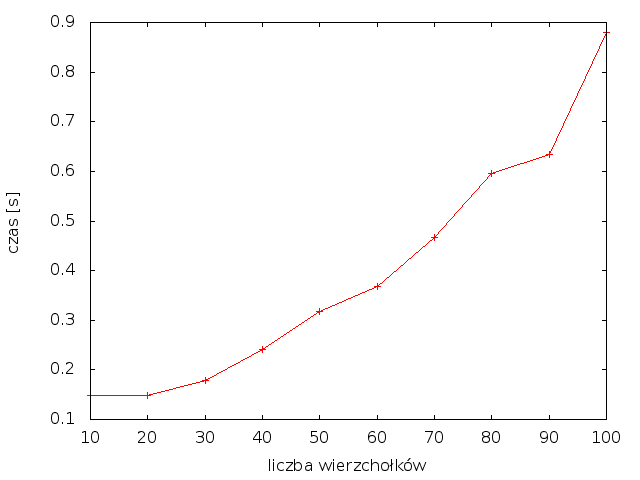
\includegraphics[scale=0.5]{results/img/den/den_01.png}
	\caption{Wykres zależności czasu wykonania od liczby wierzchołków dla grafów o gęstości 0,1}
    \end{center}
\end{figure}

\subsubsection*{Zestaw grafów o gęstości 0,2}
\begin{table}[H]
\caption{Statystyki czasowe dla zestawu grafów o gęstości 0,2}
\begin{center}
    \begin{tabular}{|l|l|l|}
    \hline
    Liczba wierzchołków & Liczba największych klik & Czas [s] \\ \hline
    10 & 9 & 0.11 \\ \hline
    20 & 1 & 0.22 \\ \hline
    30 & 5 & 0.20 \\ \hline
    40 & 5 & 0.34 \\ \hline
    50 & 10 & 0.34 \\ \hline
    60 & 22 & 0.59 \\ \hline
    70 & 1 & 0.72 \\ \hline
    80 & 1 & 0.93 \\ \hline
    90 & 4 & 1.12 \\ \hline
    100 & 10 & 1.06 \\ \hline
    \end{tabular}
\end{center}
\end{table}

\begin{figure}[h]
    \begin{center}
	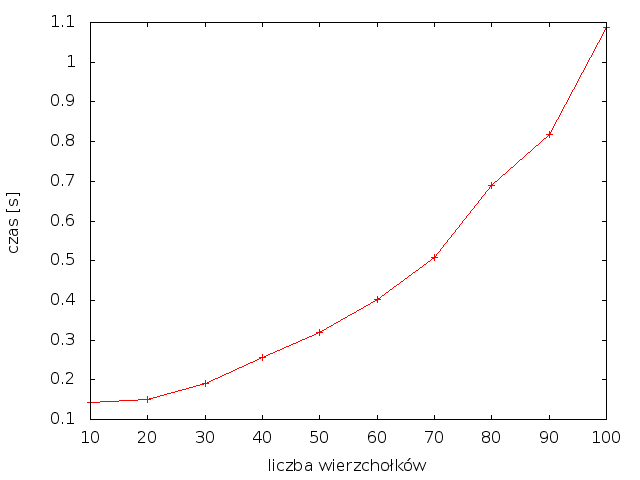
\includegraphics[scale=0.5]{results/img/den/den_02.png}
	\caption{Wykres zależności czasu wykonania od liczby wierzchołków dla grafów o gęstości 0,2}
    \end{center}
\end{figure}

\subsubsection*{Zestaw grafów o gęstości 0,3}
\begin{table}[H]
\caption{Statystyki czasowe dla zestawu grafów o gęstości 0,3}
\begin{center}
    \begin{tabular}{|l|l|l|}
    \hline
    Liczba wierzchołków & Liczba największych klik & Czas [s] \\ \hline
    10 & 3 & 0.18 \\ \hline
    20 & 2 & 0.25 \\ \hline
    30 & 20 & 0.22 \\ \hline
    40 & 1 & 0.43 \\ \hline
    50 & 1 & 0.49 \\ \hline
    60 & 29 & 0.68 \\ \hline
    70 & 1 & 1.02 \\ \hline
    80 & 2 & 1.17 \\ \hline
    90 & 8 & 1.30 \\ \hline
    100 & 9 & 1.15 \\ \hline
    \end{tabular}
\end{center}
\end{table}

\begin{figure}[h]
    \begin{center}
	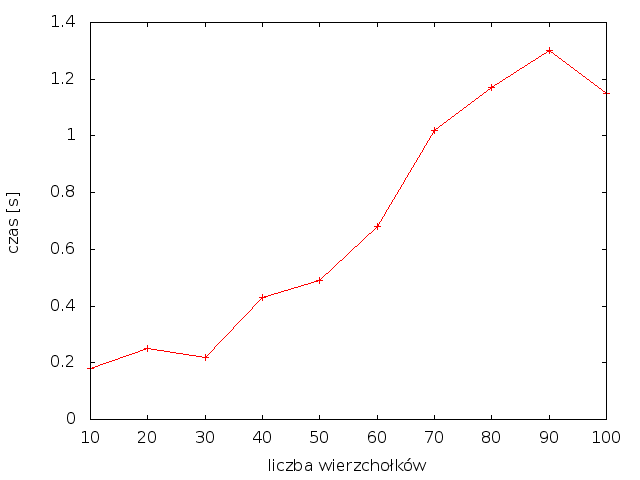
\includegraphics[scale=0.5]{results/img/den/den_03.png}
	\caption{Wykres zależności czasu wykonania od liczby wierzchołków dla grafów o gęstości 0,3}
    \end{center}
\end{figure}

\subsubsection*{Zestaw grafów o gęstości 0,4}
\begin{table}[H]
\caption{Statystyki czasowe dla zestawu grafów o gęstości 0,4}
\begin{center}
    \begin{tabular}{|l|l|l|}
    \hline
    Liczba wierzchołków & Liczba największych klik & Czas [s] \\ \hline
    10 & 7 & 0.18 \\ \hline
    20 & 10 & 0.28 \\ \hline
    30 & 6 & 0.20 \\ \hline
    40 & 6 & 0.31 \\ \hline
    50 & 10 & 0.59 \\ \hline
    60 & 32 & 0.86 \\ \hline
    70 & 5 & 1.02 \\ \hline
    80 & 5 & 1.41 \\ \hline
    90 & 9 & 1.73 \\ \hline
    100 & 49 & 1.55 \\ \hline
    \end{tabular}
\end{center}
\end{table}

\begin{figure}[h]
    \begin{center}
	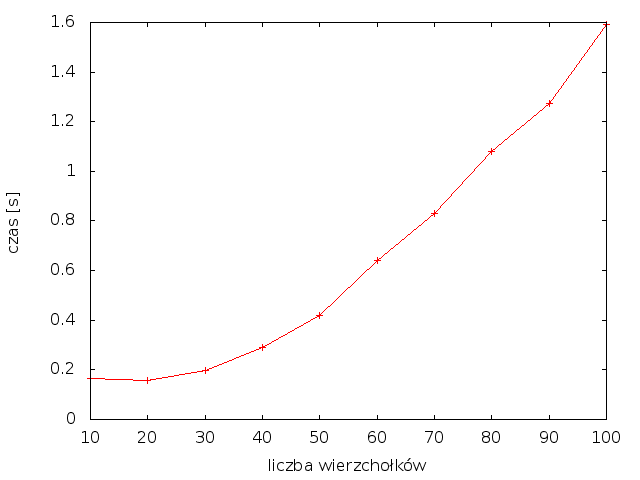
\includegraphics[scale=0.5]{results/img/den/den_04.png}
	\caption{Wykres zależności czasu wykonania od liczby wierzchołków dla grafów o gęstości 0,4}
    \end{center}
\end{figure}

\subsubsection*{Zestaw grafów o gęstości 0,5}
\begin{table}[H]
\caption{Statystyki czasowe dla zestawu grafów o gęstości 0,5}
\begin{center}
    \begin{tabular}{|l|l|l|}
    \hline
    Liczba wierzchołków & Liczba największych klik & Czas [s] \\ \hline
    10 & 12 & 0.13 \\ \hline
    20 & 3 & 0.18 \\ \hline
    30 & 11 & 0.31 \\ \hline
    40 & 2 & 0.46 \\ \hline
    50 & 3 & 0.78 \\ \hline
    60 & 4 & 1.12 \\ \hline
    70 & 7 & 1.43 \\ \hline
    80 & 7 & 1.98 \\ \hline
    90 & 2 & 2.30 \\ \hline
    100 & 17 & 2.58 \\ \hline
    \end{tabular}
\end{center}
\end{table}

\begin{figure}[h]
    \begin{center}
	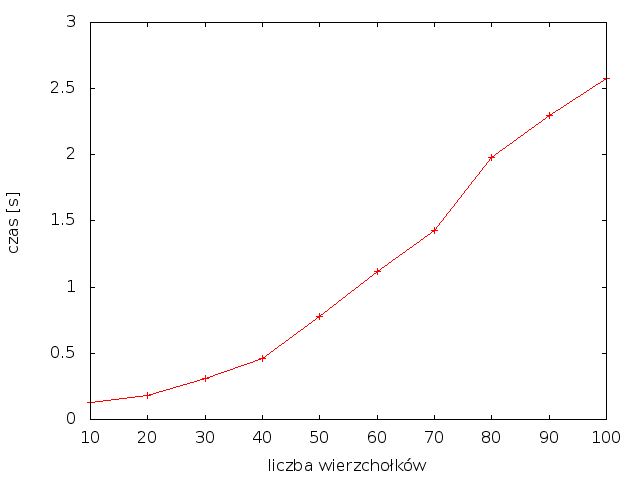
\includegraphics[scale=0.5]{results/img/den/den_05.png}
	\caption{Wykres zależności czasu wykonania od liczby wierzchołków dla grafów o gęstości 0,5}
    \end{center}
\end{figure}

\subsubsection*{Zestaw grafów o gęstości 0,6}
\begin{table}[H]
\caption{Statystyki czasowe dla zestawu grafów o gęstości 0,6}
\begin{center}
    \begin{tabular}{|l|l|l|}
    \hline
    Liczba wierzchołków & Liczba największych klik & Czas [s] \\ \hline
    10 & 1 & 0.17 \\ \hline
    20 & 3 & 0.16 \\ \hline
    30 & 15 & 0.31 \\ \hline
    40 & 1 & 0.68 \\ \hline
    50 & 1 & 1.15 \\ \hline
    60 & 34 & 1.41 \\ \hline
    70 & 5 & 2.29 \\ \hline
    80 & 1 & 2.83 \\ \hline
    90 & 3 & 3.41 \\ \hline
    100 & 48 & 2.96 \\ \hline
    \end{tabular}
\end{center}
\end{table}

\begin{figure}[h]
    \begin{center}
	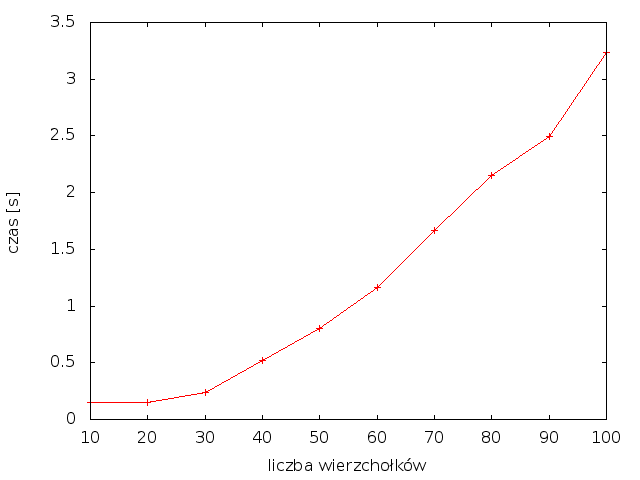
\includegraphics[scale=0.5]{results/img/den/den_06.png}
	\caption{Wykres zależności czasu wykonania od liczby wierzchołków dla grafów o gęstości 0,6}
    \end{center}
\end{figure}

\subsubsection*{Zestaw grafów o gęstości 0,7}
\begin{table}[H]
\caption{Statystyki czasowe dla zestawu grafów o gęstości 0,7}
\begin{center}
    \begin{tabular}{|l|l|l|}
    \hline
    Liczba wierzchołków & Liczba największych klik & Czas [s] \\ \hline
    10 & 4 & 0.13 \\ \hline
    20 & 2 & 0.24 \\ \hline
    30 & 23 & 0.42 \\ \hline
    40 & 2 & 0.72 \\ \hline
    50 & 16 & 1.68 \\ \hline
    60 & 24 & 2.29 \\ \hline
    70 & 1 & 3.04 \\ \hline
    80 & 92 & 4.83 \\ \hline
    90 & 39 & 8.17 \\ \hline
    100 & 52 & 13.99 \\ \hline
    \end{tabular}
\end{center}
\end{table}

\begin{figure}[h]
    \begin{center}
	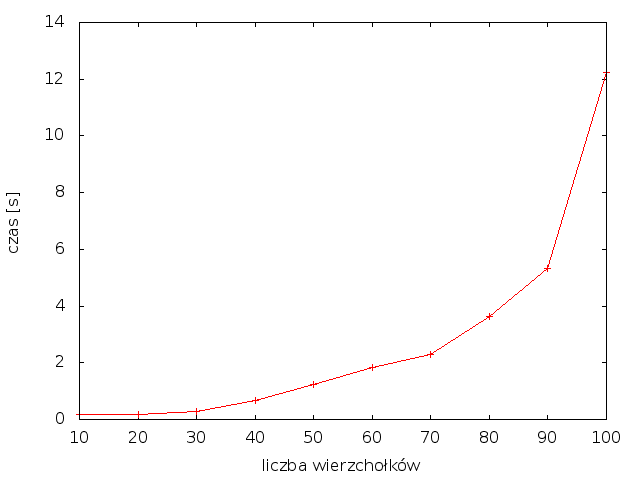
\includegraphics[scale=0.5]{results/img/den/den_07.png}
	\caption{Wykres zależności czasu wykonania od liczby wierzchołków dla grafów o gęstości 0,7}
    \end{center}
\end{figure}

\subsubsection*{Zestaw grafów o gęstości 0,8}
\begin{table}[H]
\caption{Statystyki czasowe dla zestawu grafów o gęstości 0,8}
\begin{center}
    \begin{tabular}{|l|l|l|}
    \hline
    Liczba wierzchołków & Liczba największych klik & Czas [s] \\ \hline
    10 & 3 & 0.13 \\ \hline
    20 & 38 & 0.28 \\ \hline
    30 & 15 & 0.51 \\ \hline
    40 & 2 & 1.25 \\ \hline
    50 & 47 & 2.45 \\ \hline
    60 & 17 & 3.41 \\ \hline
    70 & 5 & 7.49 \\ \hline
    80 & 9 & 18.25 \\ \hline
    90 & 58 & 63.27 \\ \hline
    100 & 29 & 174.22 \\ \hline
    \end{tabular}
\end{center}
\end{table}

\begin{figure}[h]
    \begin{center}
	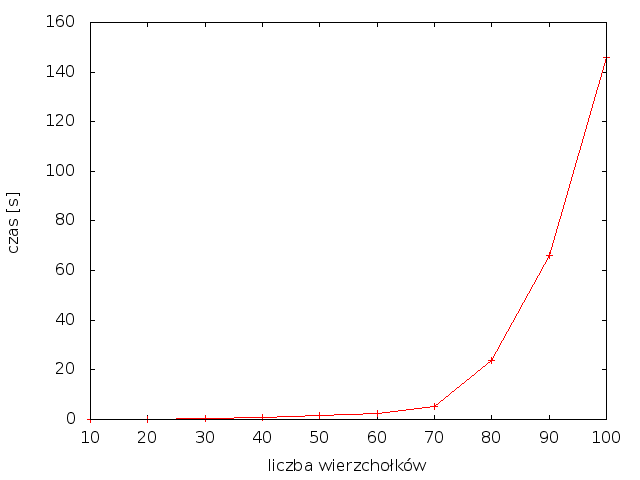
\includegraphics[scale=0.5]{results/img/den/den_08.png}
	\caption{Wykres zależności czasu wykonania od liczby wierzchołków dla grafów o gęstości 0,8}
    \end{center}
\end{figure}

\subsubsection*{Zestaw grafów o gęstości 0,9}
\begin{table}[H]
\caption{Statystyki czasowe dla zestawu grafów o gęstości 0,9}
\begin{center}
    \begin{tabular}{|l|l|l|}
    \hline
    Liczba wierzchołków & Liczba największych klik & Czas [s] \\ \hline
    10 & 2 & 0.14 \\ \hline
    20 & 2 & 0.22 \\ \hline
    30 & 2 & 0.56 \\ \hline
    40 & 5 & 1.47 \\ \hline
    50 & 30 & 2.46 \\ \hline
    60 & 67 & 11.49 \\ \hline
    70 & 127 & 102.40 \\ \hline
    80 & 106 & 437.49 \\ \hline
    90 & 204 & 3486.84 \\ \hline
    100 & 111 & 9667.70 \\ \hline
    \end{tabular}
\end{center}
\end{table}

\begin{figure}[h]
    \begin{center}
	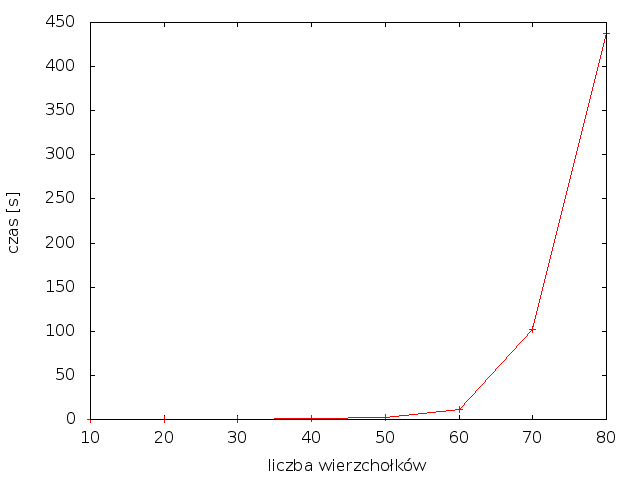
\includegraphics[scale=0.5]{results/img/den/den_09.png}
	\caption{Wykres zależności czasu wykonania od liczby wierzchołków dla grafów o gęstości 0,9}
    \end{center}
\end{figure}

\subsubsection*{Zestaw grafów pełnych}
\begin{table}[H]
\caption{Statystyki czasowe dla zestawu grafów pełnych}
\begin{center}
    \begin{tabular}{|l|l|}
    \hline
    Liczba wierzchołków & Czas [s] \\ \hline
    10 & 0.14 \\ \hline
    20 & 0.27 \\ \hline
    30 & 0.16 \\ \hline
    40 & 0.39 \\ \hline
    50 & 0.53 \\ \hline
    60 & 0.53 \\ \hline
    70 & 0.63 \\ \hline
    80 & 0.74 \\ \hline
    90 & 0.86 \\ \hline
    100 & 1.19 \\ \hline
    \end{tabular}
\end{center}
\end{table}

\begin{figure}[h]
    \begin{center}
	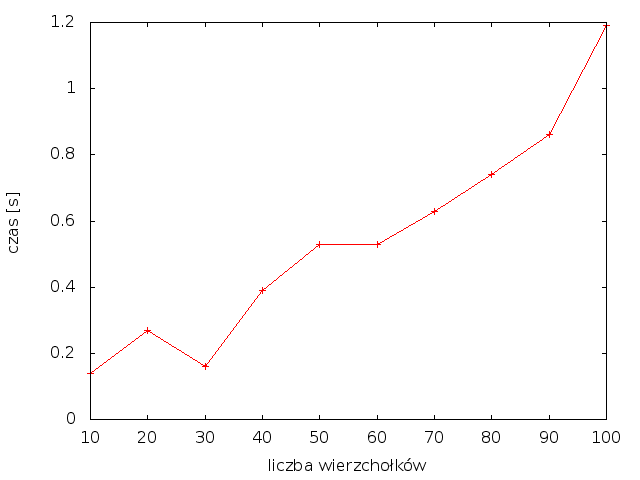
\includegraphics[scale=0.5]{results/img/den/den_1.png}
	\caption{Wykres zależności czasu wykonania od liczby wierzchołków dla grafów pełnych}
    \end{center}
\end{figure}
\newpage
\subsubsection*{Zestaw grafów o 10 wierzchołkach}
\begin{figure}[!h]
    \begin{center}
	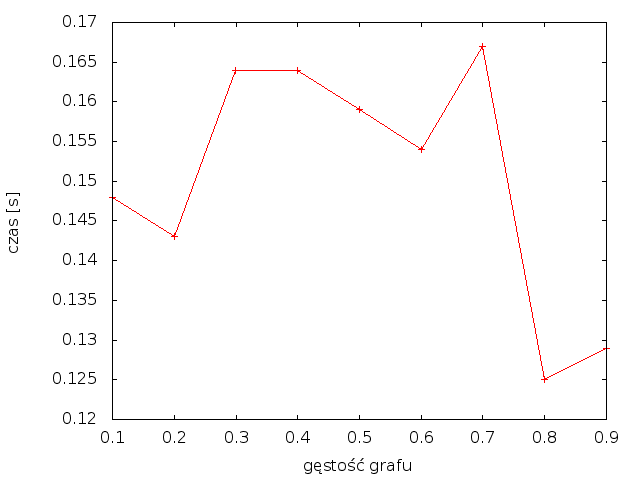
\includegraphics[scale=0.5]{results/img/dim/dim_10.png}
	\caption{Wykres zależności czasu wykonania od gęstości dla grafów o 10 wierzchołkach}
    \end{center}
\end{figure}
\FloatBarrier
\subsubsection*{Zestaw grafów o 20 wierzchołkach}
\begin{figure}[!h]
    \begin{center}
	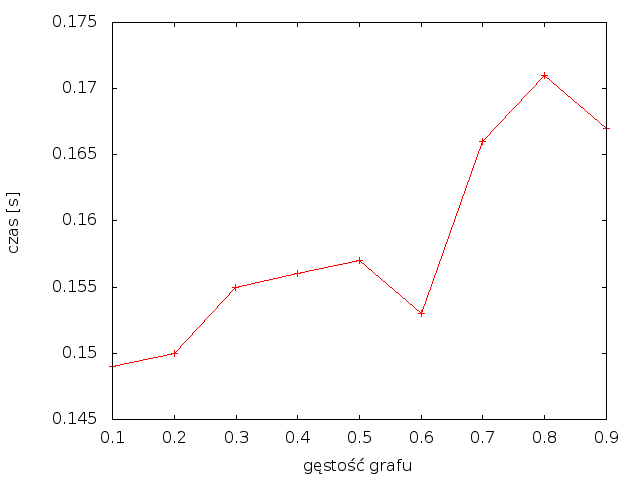
\includegraphics[scale=0.5]{results///img/dim/dim_20.png}
	\caption{Wykres zależności czasu wykonania od gęstości dla grafów o 20 wierzchołkach}
    \end{center}
\end{figure}
\FloatBarrier
\newpage
\subsubsection*{Zestaw grafów o 30 wierzchołkach}
\begin{figure}[!h]
    \begin{center}
	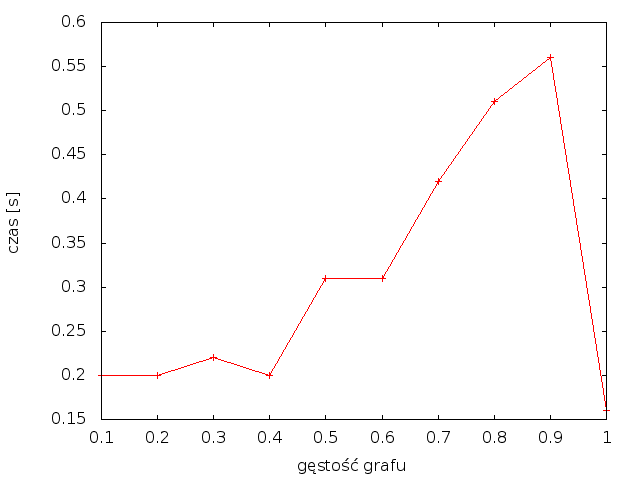
\includegraphics[scale=0.5]{results/img/dim/dim_30.png}
	\caption{Wykres zależności czasu wykonania od gęstości dla grafów o 30 wierzchołkach}
    \end{center}
\end{figure}
\FloatBarrier
\subsubsection*{Zestaw grafów o 40 wierzchołkach}
\begin{figure}[!h]
    \begin{center}
	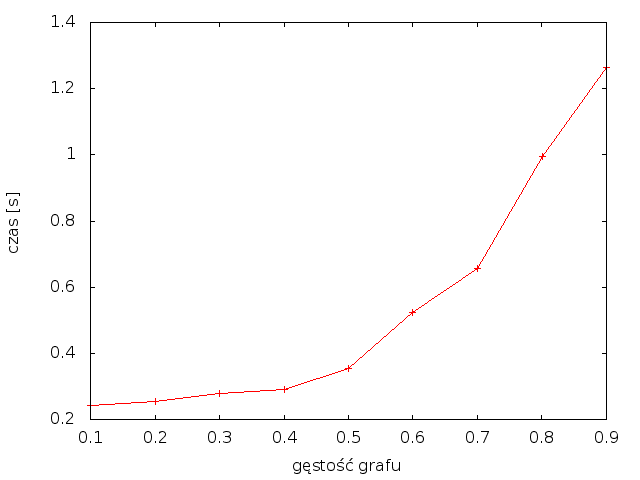
\includegraphics[scale=0.5]{results/img/dim/dim_40.png}
	\caption{Wykres zależności czasu wykonania od gęstości dla grafów o 40 wierzchołkach}
    \end{center}
\end{figure}
\FloatBarrier
\newpage
\subsubsection*{Zestaw grafów o 50 wierzchołkach}
\begin{figure}[!h]
    \begin{center}
	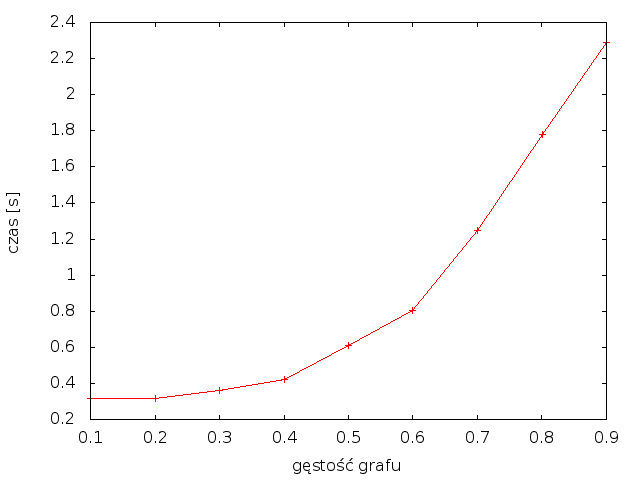
\includegraphics[scale=0.5]{results/img/dim/dim_50.png}
	\caption{Wykres zależności czasu wykonania od gęstości dla grafów o 50 wierzchołkach}
    \end{center}
\end{figure}
\FloatBarrier
\subsubsection*{Zestaw grafów o 60 wierzchołkach}
\begin{figure}[!h]
    \begin{center}
	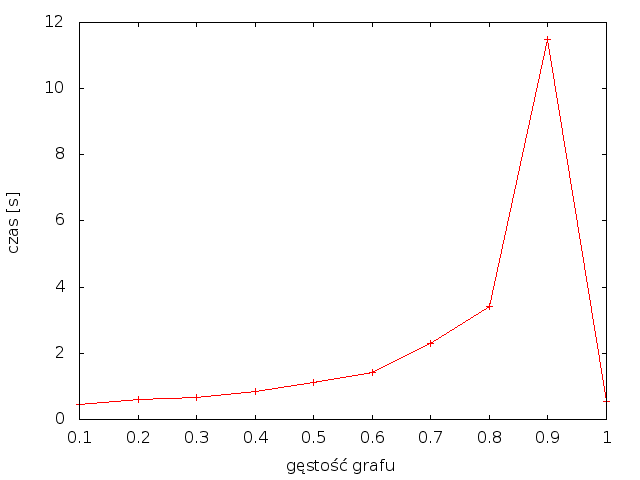
\includegraphics[scale=0.5]{results/img/dim/dim_60.png}
	\caption{Wykres zależności czasu wykonania od gęstości dla grafów o 60 wierzchołkach}
    \end{center}
\end{figure}
\FloatBarrier
\newpage
\subsubsection*{Zestaw grafów o 70 wierzchołkach}
\begin{figure}[!h]
    \begin{center}
	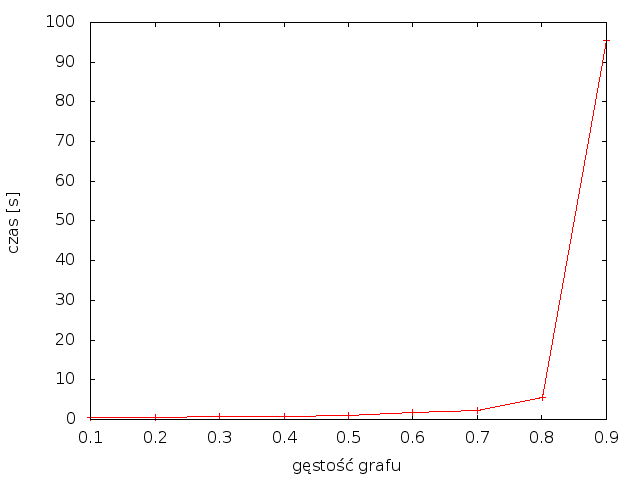
\includegraphics[scale=0.5]{results//img/dim/dim_70.png}
	\caption{Wykres zależności czasu wykonania od gęstości dla grafów o 70 wierzchołkach}
    \end{center}
\end{figure}
\FloatBarrier
\subsubsection*{Zestaw grafów o 80 wierzchołkach}
\begin{figure}[!h]
    \begin{center}
	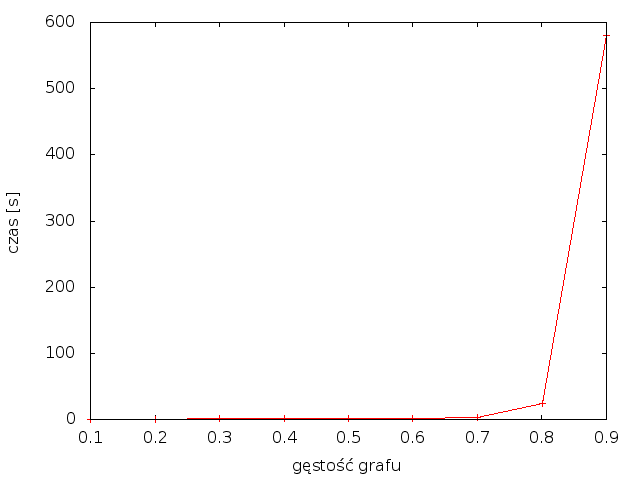
\includegraphics[scale=0.5]{results/img/dim/dim_80.png}
	\caption{Wykres zależności czasu wykonania od gęstości dla grafów o 80 wierzchołkach}
    \end{center}
\end{figure}
\FloatBarrier
\newpage
\subsubsection*{Zestaw grafów o 90 wierzchołkach}
\begin{figure}[!h]
    \begin{center}
	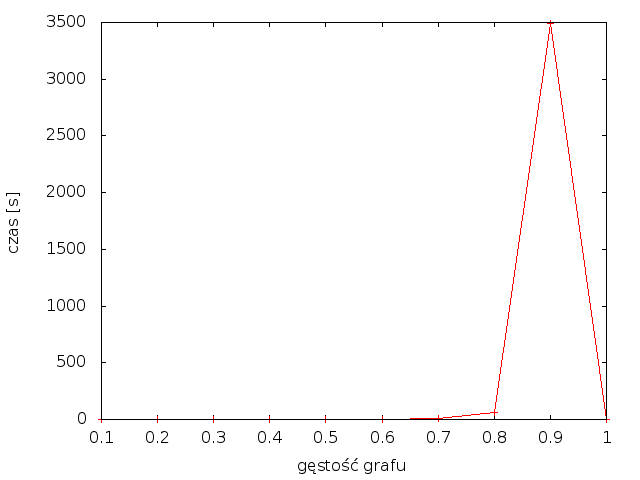
\includegraphics[scale=0.5]{results/img/dim/dim_90.png}
	\caption{Wykres zależności czasu wykonania od gęstości dla grafów o 90 wierzchołkach}
    \end{center}
\end{figure}
\FloatBarrier
\subsubsection*{Zestaw grafów o 100 wierzchołkach}
\begin{figure}[!h]
    \begin{center}
	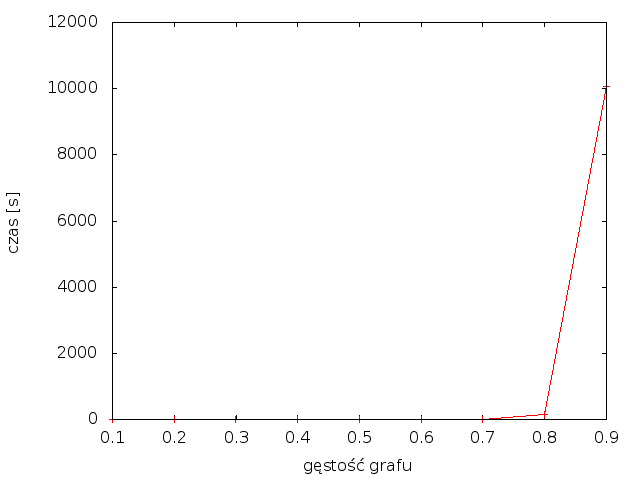
\includegraphics[scale=0.5]{results/img/dim/dim_100.png}
	\caption{Wykres zależności czasu wykonania od gęstości dla grafów o 100 wierzchołkach}
    \end{center}
\end{figure}
\FloatBarrier

\section{Podsumowanie i wnioski}
W ramach projektu zrealizowana została aplikacja umożliwiająca znalezienie największej kliki w zadanym grafie. 
Zaimplementowany algorytm został przetestowany pod kątem poprawnego działania jak również wykonane 
zostały badania mające na celu zbadanie jego zachowania dla grafów o zróżnicowanej gęstości.

W wyniku eksperymentu przeprowadzonego na zestawie grafów losowych obejmującego grafy o liczbie wierzchołków 
10, 20, 30, 40, 50, 60, 70, 80, 100 oraz gęstościach z przedziału 0,1 -- 1 uzyskano rezultaty czasowe zaprezentowane w rozdziale \ref{testy}.

Analizując otrzymane wyniki można zauważyć, iż dla grafów o gęstościach z przedziału 0,1 -- 0,6 czas wykonania
wzrasta w sposób zbliżony do liniowego wraz ze wzrostem liczby wierzchołków grafu. 
Odmienna sytuacja ma miejsce dla grafów o gęstości z przedziału 0,7 -- 0,9, dla których czas wykonania 
algorytmu rośnie wykładniczo wraz ze wzrostem liczby wierzchołków. 
Prawidłowość ta jest szczególnie widoczna dla grafów o gęstości 0,9. 

Osobną klasę grafów stanowią grafy pełne, dla których czasy wykonania zależą, podobnie jak w przypadku grafów rzadkich, 
w sposób zbliżony do liniowego od liczby wierzchołków.

Na podstawie analizy wyników można stwierdzić, że zaimplementowany algorytm silnie zależy 
zarówno od rozmiaru grafu jak i jego gęstości. W przypadku grafów rzadkich oraz pełnych czasy uzyskiwane przez
 algorytm nie przekroczyły kilku sekund dla grafów o 100 wierzchołkach. 
Niestety, w przypadku jednocześnie dużej gęstości i liczby wierzchołków grafu ujawnia się wykładnicza złożoność 
algorytmu i czas działania drastycznie wzrasta (czego przykładem jest wynik dla grafu o 100 wierzchołkach
i gęstości 0,9 sięgający prawie 3 godzin).
\begin{appendices}
\section{Zawartość katalogów}

Opis zawartości poszczególnych katalogów:

\begin{itemize}
 \item \texttt{gis-kliki-java} - implementacja algorytmu będącego przedmiotem projektu,
 \item \texttt{gis-c} - pomocniczy program generujący rozwiązania referencyjne z wykorzystaniem biblioteki igraph,
 \item \texttt{tests} - pliki dla testów weryfikujących poprawność implementacji:
 	\begin{itemize}
 		\item \texttt{correctness} - pliki z grafami wykorzystanymi do weryfikacji poprawności algorytmu,
 		\item \texttt{performance} - pliki z grafami wykorzystanymi podczas analizy czasów wykonania algorytmu i jego poprawności,
 	\end{itemize}
 \item \texttt{doc} - dokumentacja projektu.
\end{itemize}

\section{Instrukcja obsługi}

Aplikacja działa w trybie konsolowym. W celu jej uruchomienia należy wykonać następujące kroki:
\begin{enumerate}
 \item Skompilować kod Javy. W tym celu wystarczy uruchomić skrypt \texttt{gis-kliki-java/build.sh}.
 \item Przygotować pliki wejściowe.
 \item Uruchomić program jednym z możliwych sposobów:
 \begin{itemize}
 	\item Ręczne uruchomienie. W katalogu \texttt{gis-kliki-java} należy wykonać następujące polecenie: \\
 	\texttt{java -cp bin main/Main < plik\_wejściowy}
 	\item Uruchomienie z wykorzystaniem skryptu.
 	Wraz z programem dostarczone są dwa skrypty ułatwiające uruchamianie i testowanie aplikacji:
 	\begin{itemize}
 		\item \texttt{run\_basic.sh} \\
 		W wyniku działania zwracany jest czas wykonania oraz znaleziona największa klika.\\
 		Przykład wykorzystania:
 		\texttt{run\_test.sh graf1\_in.txt graf2\_in.txt} (na wejście można przekazać wiele plików)
 		\item \texttt{run\_test.sh} \\
 		Skrypt umożliwia działanie aplikacji w dwóch trybach: standardowym (jak w przypadku \texttt{run\_basic.sh}) 
oraz rozszerzonym, weryfikującym znalezione rozwiązanie z rozwiązaniami referencyjnymi. 
Jeśli plik wejściowy nazywał się np. \texttt{123\_in.txt}, to skrypt poszukuje rozwiązania w pliku o nazwie \texttt{123\_out.txt}. 
W przypadku nie znalezienia pliku z rozwiązaniem aplikacja zostaje uruchomiona w trybie standardowym. \\
 		Przykład wykorzystania:
 		\texttt{run\_test.sh graf1\_in.txt graf2\_in.txt} (na wejście można przekazać wiele plików)
 	\end{itemize}
 \end{itemize}
\end{enumerate}

\end{appendices}

\bibliographystyle{plain}
\bibliography{references}
\end{document}
